\documentclass[11pt, a4paper]{report}
\usepackage{syntonly}
\usepackage[utf8]{inputenc}
\usepackage[backend=biber]{biblatex}
\addbibresource{mybib.bib}
\usepackage{hyperref}
\usepackage{graphicx}
\usepackage{color}
\usepackage{framed}
\usepackage{subcaption}
\usepackage{float}
\graphicspath{ {images/} }
\usepackage{svg}
\usepackage{pdfpages}
\usepackage{blindtext}
\usepackage{mathtools}
\usepackage{amssymb}
\usepackage{amsbsy}
\usepackage{amsfonts}
\usepackage{amsthm}
\usepackage{amsmath}
\usepackage{bm} %\bm
\usepackage{IEEEtrantools}
\usepackage[section]{placeins} %\Floatbarrier
\usepackage{float}
\usepackage{verbatim}
\usepackage[a4paper, width=150mm, top=25mm, bottom=25mm]{geometry}
\usepackage{fancyhdr}
\hypersetup{linktocpage,
            linktoc=all,
            %colorlinks=true,
            %linkcolor=blue,
}

\pagestyle{fancy}
\fancyhf{}
\fancyhead[C]{\rightmark}
\fancyfoot[C]{\thepage}

\setlength{\parskip}{1.0em}
\setlength{\parindent}{1em}

\usepackage{lipsum}

\theoremstyle{plain}
\newtheorem{theorem}{Theorem}[chapter]
\newtheorem{lemma}[theorem]{Lemma}

\theoremstyle{definition}
\newtheorem{mydef}{Definition}[chapter]

\theoremstyle{remark}
\newtheorem{remark}{Remark}[chapter]


%newcommands
\newcommand{\N}{\mathbb{N}}
\newcommand{\C}{\mathbb{C}}
\newcommand{\R}{\mathbb{R}}
%\newcommand{\Z}{\mathbb{Z}}
\newcommand{\F}{\mathbb{F}}
\newcommand{\E}{\mathbf{E}}
\newcommand{\X}{\mathbf{X}}
\newcommand{\x}{\mathbf{x}}
\newcommand{\Z}{\mathbf{Z}}
\newcommand{\z}{\mathbf{z}}
\newcommand{\Y}{\mathbf{Y}}
\newcommand{\y}{\mathbf{y}}
\newcommand{\W}{\mathbf{W}}
\newcommand{\w}{\mathbf{w}}
\newcommand{\DD}{\mathbf{D}}
\newcommand{\dd}{\mathbf{d}}
\newcommand{\LL}{\mathcal{L}}
\newcommand{\NN}{\mathcal{N}}
%\newcommand{\B}{\{-1,1\}}
%\newcommand{\bvec}[1]{\mathbf{#1}}
%\newcommand{\bv}[1]{\mathbf{#1}}
%\newcommand{\b}[1]{\boldsymbol{#1}}
\newcommand{\bv}[1]{\boldsymbol{#1}}
\newcommand{\bvec}[1]{\boldsymbol{#1}}
\newcommand{\ceil}[1]{\lceil{#1}\rceil}
\newcommand{\floor}[1]{\lfloor{#1}\rfloor}
\newcommand{\gt}{>}
\newcommand{\lt}{<}
\newcommand{\tuple}[1]{\langle #1 \rangle}

%\floatstyle{ruled}
\floatstyle{boxed}
\restylefloat{figure}
\restylefloat{table}
%\pagestyle{fancy}

\begin{document}

\begin{titlepage}
\begin{center}
{
\includegraphics[width=1.0\textwidth]{images/MPIMG_RGB_gruen.png}}\\
\vspace*{1cm}
%\vfill
\Large
%$\mathrlap{\text{sc}{\ast}$ GMV\AE
%\textbf{scGMV\AE}
%$\mathrlap{\mathrm{sc}}{\ast}$GMV\AE
$\mathrm{sc}\ast$GMV\AE
%\textbf{$\mathclap{sc}{\ast}$GMV\AE}
%\textbf{{\ae}g$\mathllap{sc}{\ast}$cGMV\AE}
%\textbf{{\ae}g$\text{sc}{\ast}$cGMV\AE}\\
%%\normalsize \textbf{{\ae}g$\text{sc}{\ast}$cGMV\AE} stands for\\
%\textbf{A}nalysis \textbf{E}ncoding and \textbf{G}eneration of 
%\textbf{S}ingell cell RNASeq and whatever 
%$\bf{\ast}$ with \textbf{C}onditional \textbf{G}aussian 
%\textbf{M}ixture \textbf{V}ariation \textbf{A}uto\textbf{E}ncoders. 
%\vfill

%\vspace{0.5cm}


%\normalsize
\large
a Master Thesis in Bioinformatics
\vspace{1.0cm}

Thesis advisor / 1st Supervisor: professor Martin Vingron\\
2nd Supervisor: professor Tim Conrad

\vfill

Yiftach Josef Kolb
(Matrikelnummer 5195763)
%\normalsize{(Matrikelnummer 5195763)}

Berlin, \today

\vfill
{
\includegraphics[width=0.8\textwidth]{images/fu-logo_bildschirm_RGB1.jpg}}
\end{center}
\normalsize
\end{titlepage}


\includepdf[pages=-,
scale=.8,
%pagecommand=\chapter*{Declaration},
linktodoc=true,
]{./Selbstaendigkeitserklaerung_EN-Flattened.pdf}


\chapter*{Abstract}
Single cells RNASeq data (scRNASeq) can be thought of as coming from a conditional mixture distribution, where
the categories indicate cell types and the conditions indicate either technical
batches or post/pre--exposure effects.
In this thesis we take the GMVAE (Gaussian mixture variational autoencoder) model~\cite{dilokthanakul2016deep},
introduce some modifications to the underlying probabilistic model
and test its suitability for analysis, embedding and generation of scRNASeq
data.
We think that the model is particularly suitable for (semi)supervised use case,
where information on the cell types of the dataset is partially available.
$\text{sc}{\ast}$GMVAE stands for 
"Single cell RNASeq ($\ast$) Conditional Gaussian Mixture Variation
AutoEncoder".

\chapter*{Acknowledgement}

I am very thankful to
professor Martin Vingron for 
for being my mentor and advisor and for directing me through this work. 
I owe Martin, his department and the Max Planck institute  a lot of gratitude
for providing me a very welcoming, productive and scientifically rich
environment.
Thanks to professor Tim Conrad for being my thesis defense supervisor twice in a
row!


%\listoftables

\listoffigures

\tableofcontents


\chapter*{Preface}

This thesis could be colloquially summarized by:
\emph{VAEs -- why should we (bioinormarticians) care about them}.


\chapter{Notations and definitions, preliminary concepts}

\section{Tensors, shape, axis, dimension}
In machine learning one often encounters data structures that have
multi-dimensional \emph{shape} which we call \emph{tensors}. For example a 28
over 28 color image can be represented as a 3-dimensional shape ($3,28, 28)$
representing pixel's RGB channels (AKA its color), its height, and its
width. This creates some
confusion as to what one means by "dimensions"-- the dimensions of the data shape
which is $3$,
or the number of dimensions of the data content (for lack of a better term),
which is  $3 \times 28 \times 28$. For example a vector $\x \in \R^5$
is represented as a 1 dimensional shape but it has $5$ \emph{dimensions in
total}. Similarly the color image has a $3$ dimensional shape but it has $28
\cdot 28 \cdot 3$ dimensions in total. It has 3 \emph{axes}, whose respective
sizes are $28$, $28$, and $3$. 

A (real valued) \emph{tensor} is an element of a tensor product space, for
example the color image described above, $\x \in  \R^{28 \times 28 \times 3}
\triangleq \R^{28} \otimes \R^{28} \otimes \R^3$. A \emph{tensor} has $0$ or
more axes and it generalizes scalar, vector, matrix and higher dimensional
shaped entities.

In Pytorch~\cite{pytorch2018pytorch} terminology \emph{dimension} is used for the
number of axes (data shape) but it is inconsistent with the way dimension is used in
mathematics with regards to vectors which is the number of entries (data
content size). 
We suggest that \emph{dimension} should only refer to data content size,  
and \emph{shape size} to the number of axes it comes in. So for the same $\x$ color
image: $\text{dim}(\x) = 3 \times 28 \times 28$ and $\text{shape}(\x) =
(3,28,28)$ and $\text{shape size}(\x) = \text{axes}(\x) = 3$.

\begin{mydef}
\label{def:tensor}
A \emph{scalar} $x \in \R$ is an element of the (real) field. It has $0$
\emph{dimensions}, $0$ \emph{axes} and \emph{shape} $(,)$.

A \emph{vector} $\x \in \R^n$ has $n$ dimensions, $1$ axis, and shape $(n,)$.

A matrix $\X \in \R^{m \times n}$ has $mn$ dimensions (in total), $2$ axes, and
shape of $(m,n)$. Its first and second axes are said to be of sizes $m$ and $n$
respectively.

A tensor $\x \in \R^{n_1 \times \dots \times n_k}$ has $\prod_1^k n_i$
dimensions, $k$ axes, and shape $(n_1, \dots, n_k)$. Its $i$'s axis is said to
be of size $n_i$.
\end{mydef}

In practice a tensor $\x \in \R^{n_1 \times \dots \times n_k}$ is represented as
a $k$ dimensional array. We call its first axis the \emph{row axis} or
alternatively when we want to emphasize that this is a collection of several
tensors, the \emph{batch axis}. The tensor $\x_i = \x[i]$, which is the $k-1$
dimensional sub-array with the first coordinate held fixed, is called the
\emph{$i$'th row} of $\x$. Sometimes we want to represent a tensor $\x$ as a
collections of tensors. For example it can represent a collection of several
images. Each "row" then represents an image tensor.

It may be that our data set comes not as one tensor but in several tensors. For
example we might have a tensor $\x$ representing an ordered set of images, and a
tensor $\y$ which represents the category of each image. Because they have
different shapes they don't fit together in one tensor. However since they refer
to the same entities (images) their first axes have equal sizes. We use the
notation $(\x, \y)$ to denote the matching pairs of image/category, implicitly
requiring them to have equally sized first axes.

If $\x,\y$ have the same number of axes and their respective axes sizes are
equal on all but the last axis then we can concatenate them by "stacking" $\y$
on top of $\x$ along the last axis.

\begin{mydef}
\label{def:rowrep}
If $\x$ is a tensor, $\x_i$ represents the $i$'th "row" of $\x$,
and $\x = \{\x_1, \dots , \x_n\}$ is the \emph{row representation} or 
\emph{batch
representation} of $\x$.
\end{mydef}

\begin{mydef}
\label{def:pairnotaion}
Let $\x, \y$ be tensors whose first axes have equal dimensions, $n$. Then $(\x, \y)$
is the set of ordered pairs $(\x,\y) \triangleq \{(\x_i,\y_i) : i=1 \dots n\}$.
\end{mydef}

\begin{mydef}
\label{def:concat}
If $\x,\y$ have the same number of axes and equal dimension on all but their last axis, 
the $(\x|\y)$ is their concatenation on the last axis. 
\end{mydef}

%\boldmath
\section{samples, batches, mean-sum rule}

We distinguish between two types of tensors depending on what they represent.
Let $\x \in \R^{m \times n \times l}$ be a tensor. If we say that $\x$ is a
\emph{sample} or a \emph{data point} it means it is a single sample from our
data set. If we say that it is a \emph{batch}, then it represent a collection of
$m$ samples. In this case the first axis is the batch axis and the rest of the
axes are the sample axes.

As a rule the default reduction is summation over sample axes and mean over the
batch axes. For example if $\x$ is a sample, then $\|\x \|_1 = \sum_i \sum_j
\sum_k |x_{i,j,k}|$ because it has no batch axis. If $\x$ is a batch, then we
take the mean over the first axis: $\| \x \|_1 = \frac{1}{m} \sum_i \| \x_i \|_1
= \frac{1}{m} \sum_i \sum_j \sum_k |x_{i,j,k}|$.

The reason that we do that is that for batches, we want batches of different
sizes to be comparable so it is straight forward to take mean. For the other
axes, as we will see in the case of VAE we use the ELBO function where we have
to sum over the sample axes.

\label{meansumrule}


\section{Matrices and vectors}

The type of data we work with in this paper can be represented as vectors. For
example images of shape $(h,w,c)$ can be flattened into a single axis shape $(h
\cdot w \cdot c,)$ vector.

Throughout this paper (modulo typing errors) we use capital bold math Latin or
Greek letters ($\bv{X, \Sigma}$) to represent matrices. To stress that we talk
about matrices rather than vectors we show product ($\times$) in the dimension,
i.e $\bv{X} \in \R^{m \times n}$. Although technically the matrix--space is the
tensor product $\R^m \otimes \R^n$.

Bold small math letters ($\bv{x}$) represent usually row vectors, but in cases
where it makes sense may also represent matrices such as a batch of several
vectors (each row is a different data point). In few occasions it makes sense to
let it represent both a matrix and a vector, for example, $\bv{\sigma}$ may
represent both the covariance matrix and the variance vector of a diagonal
Gaussian distribution. Non-bold math letters ($x, \sigma$, \dots) may represent
scalar or vectors in some cases and hopefully it is clear from the context or
explicitly stated.

Since we are only dealing with real matrices the transpose and the conjugation
operators are the same ($A^T = A^*$) but over $\C$ conjugation is usually the
"natural" operation and we use it to indicate that some property is still valid
over $\C$ with conjugation.

Sometimes matrices are given in row/column/block notations inside brackets where
the elements are concatenated in a way that makes positional sense. For example
both $(\x,\y)$ and $(\x | \y)$ represent a matrix with 2 \textbf{columns}.

As mentioned usually just $\x$ means a column vector and $\x^T$ means a row
vector but sometimes in matrix notation $\x$ represents a row when it makes
sense. We use \textbf{curly} brackets to indicate the \textbf{row}
representations of a matrix. For example $\{\x, \y\}$ represents a matrix whose
\textbf{rows} are $\x$ and $\y$ (as row vectors), which alternatively could be
represented as $(\x, \y)^T$ (and symmetrically $(\x,\y) = \{\x,\y\}^T$).

$(\X,\Y)$ or $(\X | \Y)$ represent concatenation of two matrices along the
second axis (concatenation of rows) which implicitly means they have the same
number of rows. $\{\X, \Y\}$ represents concatenation along the first axis
(concatenation of columns) which implies they must have equal number of columns.

Zero--blocks are indicated with $0$ or are simply left as voids. For
example
$ \left( \begin{array}{c c} \bv{A} & \bv{B} \\ \bv{0} & \bv{D}
\end{array} \right) $ 
,
$ \left( \begin{array}{c c} \bv{A} & \bv{B} \\  & \bv{D}
\end{array} \right) $ 
both represent block notation of the same upper--triangular matrix.

\begin{mydef}
Let $\X = \{\x_1, \dots \x_m\} \in \R^{m \times n}$
be a matrix in \textbf{row} notation. Then its \emph{squared Frobenius norm} is
\begin{equation}
\label{def:frobnorm}
\|X\|_F^2 \triangleq \text{trace}(\X \X^*) 
= \sum_{i=1}^{m} \|\x_i\|^2_2 = \sum_{i=1}^m \sum_{j=1}^n x_{ij}^2
\end{equation}
\end{mydef}



\section{Functions and maps}
%see~\ref{meansumrule}
\label{seq:functions}
Functions are usually understood to be scalar, namely $f:\R^n \to \R$ while maps
are more general $g:\R^n \to \R^m$. When we say that a map (or function) $\phi
:\R^n \to \R^m$ is \emph{parameterized}, it implicitly means that $\phi$ has
additional variables which we treat as parameters $\phi_{\w}(\x) = \phi(\x, \w)$
where $\x \in \R^n$ and $\w$ is the function's parameter set which we don't always specify
its domain and we may not always subscript $\phi$ with it. The parameterized map
$\phi$ itself may be identified with its parameter set and then both are
designated with $\phi$.
It is important to stress out that the
parameterization is not just an enumeration of the functions in our class, rather we 
want $\w$ to come from some domain and that the parameterized function
$\phi(\x,\w)$ should be \emph{differentiable in its parameters} $\w$.
It is of lesser concern whether $\phi$ is also differentiable in $\x$.
For example a classifier is a discrete function over $\x$ so a neural network
$\phi$ that classifies $\x$ is not differentiable in $\x$ but it is on its
parameters $\w$.

In the context of neural networks, when we say \emph{linear} map, we actually
mean an \emph{affine} map. An affine map $f(x_1 \dots x_n)$ can always be
represented as a linear map with one extra variable which is held fixed $x_0
\equiv 1$: $f(x_0, \dots x_n) = b + a_1 x_1 + \dots a_n x_n$. We call $b$ the
\emph{bias} of the linear map $f$.
\label{affinelinear}

\section{Data types}
We assume that the input data unless otherwise stated is real-valued matrix.
Rows represent \emph{samples} and columns represent \emph{variables}. We assume
that each row is a realization of a random vector. If we have $N$ rows, then the
corresponding $N$ random vectors are assumed to be independent. So depending on
the context, when we say observation, or row, we may mean the actual observed
values, or to the random vector which was realized by said observation.

We deal with two kinds of datasets in this thesis. One of them is Single cell
RNASeq data. This kind of data represents gene expression levels in individual
cells, where rows represent cells and columns represent genes. So if we see a
reading of $0.5$ in row $2$ column $4$ in means that in cell $2$ gene $4$ has
normalized expression of $0.5$.

The other kind of data is images. For example the MNIST data set contains
greyscale $28 \times 28$ images of hand written digits. We still think of such
data set as a matrix. The first axis always represents the samples, so each
"row" represent an image. The rest of the axes represent the image.
Alternatively we can also flatten the images into one axis and think of an image
as a row vector of $28*28$ dimensions.

There could possibly be additional data matrices with information about class or
conditions. We use \emph{one-hot encoding} to represent such information. For
example in the case of the MNIST dataset every image also comes with a label
which indicates what digit it is. Since there are $10$ digits ($0$ to $9$) the
class matrix is going to have $10$ columns and each row is a one-hot vector
indicating the digit of the corresponding image.

\begin{mydef}
\label{def:datamatrix}
A \emph{data matrix} is a real--valued matrix $\bv{X} \in \R^{N \times n}$ which
represents a set of $N$ $n$-dimensional data points. The $N$ rows are also
called \emph{observations} and the $n$ columns are \emph{variables}.
\end{mydef}

\begin{mydef}
\label{def:classmatrix}
A \emph{class matrix}, or also a \emph{condition matrix} $\bv{C} \in \R^{\N
\times c}$ is a real matrix which represents one-hot encoding of $c$ classes or
conditions over $N$ samples. For example if sample $i$ has class $j$, then
$(\forall k\in 1, \dots, c) \bv{C}[i,k] = \delta_{jk}$.

We say that that $\bv{C}$ is a \emph{class probability matrix} or a
\emph{relaxed class matrix} (same with condition) if instead of being one-hot
its rows are distributions---each row is non-negative and sums up to $1$.
\end{mydef}

Usually if the input data includes class/condition information, it comes as a
class matrix (pure one-hot) but the output (the prediction) is naturally
probabilistic and hence is relaxed.

\subsection{Input set and target set}
Our data usually comes in several, two or more matrices,
and when it does, the rows of these matrices are paired (or tupled if they are
more than 2).
For example we could have an input data $\X$ and a target data $\Y$, representing 
samples from some unknown function $f(\x) = \y$ that we want to learn. 
This is generally how things are in an image classification task,
where $\X$ may be a set of images, and $\Y$ is
their labels. Implicitly $\X,\Y$ must have the same number of rows. And when we
speak about paired input/target $\x,\y$ it means some $(\x,\y) \in (\X,\Y)$ and
$\x,\y$ belong to the same sample (same row number).

%In the case of autoencoders, the target set is also the input set and $f$ is the
%identity (in this case $f$ is known but we want to learn an efficient way
%to represent the data).

%For example it could be a single cell RNASeq data
%with normalized gene expression data $\X$,  cell types as target
%matrix $\Y$. 

\subsection{Probabilistic interpretation of the data}
Suppose that we have a data matrix $\X = \{\x_1, \dots , \x_N\}$. We think of
$\X$ as a set of $N$ independent samples, all drawn from the same data
distribution $\x \sim p(\x)$. We think of $\x_i$ as a realization of a random
vector which we also denote with $\x_i$. The random vectors $\x_i$ are
iid we designate with by $\x$ a 'generic' random vector with the same
distribution. This is another motivation why
we take mean over the batch dimension, because then $\|\X\| = \frac{1}{N}
\sum_1^N \|\x_i\| \approx \E [\|\x\|]$.


\section{Linear algebra preliminary: SVD and PCA}
In the following we state some facts and bring without proof what are the singular
value decomposition and the principle components of a matrix. For a full proof
see~\cite{serre2001matrices}.

%\section{SVD and PCA}
Let $\bv{X} \in \R^{N \times n}$ be a real-valued matrix representing $N$
samples of some $n$-dimensional data points and let $r= \text{rank}(\bv{X}) \leq
\min(n,N)$. 

$\X \X^*$ and $\X^* \X$ are both symmetric and positive semi-definite
(since we are only dealing with real-valued data $\X^* = \X^T$). Their
eigenvalues are non-negative, and they both have the same positive eigenvalues,
exactly $r$ such, which we mark $s_1^2 \geq s_2^2 \geq \dots s_r^2 \gt 0$. The
values $s_1 \dots s_r$ are called the \emph{singular values} of $\bv{X}$.

Let $\bv{S} = 
\begin{pmatrix}
s_1 & & &\\
& s_2 & &\\
& & \ddots &\\
& & & s_r
\end{pmatrix} \in \R^{r \times r}
$

Let $\bv{U} = (\bv{u}_1 | \dots | \bv{u}_N) \in \R^{N \times N}$ be the (column)
right eigenvectors of $\X \X^*$ sorted by their eigenvalues. Then $\bv{U} =
(\bv{U}_r, \bv{U}_k)$ where $\bv{U}_r = (\bv{u}_1 | \dots | \bv{u}_r) \ \in
\R^{N \times r}$ are the first $r$ eigenvectors corresponding to the non-zero
eigenvalues, and $\bv{U}_k$ are the eigenvectors corresponding to the $N-r$
$0$-eigenvalues. Similarly let $\bv{V}  = (\bv{V}_r, \bv{V}_k)\in \R^{n \times
n}$ be the (column) right eigenvectors of $\X^* \X$, sorted by the eigenvalues,
where $\bv{V}_r  = (\bv{v}_1 | \dots | \bv{v}_r) \in \R^{n \times r}$ are the
firs $r$ eigenvalues and $\bv{V}_k$ are the $n-r$ null-eigenvectors.

The critical observations is that $\bv{V}_r = \bv{X}^* \bv{U}_r S^{-1}$ and then
$\bv{U}_r^* \X \bv{V}_r = S$.

The \textit{singular value decomposition (SVD)} of $\X$ is 

\begin{equation}
\label{eq:svd}
\X = \bv{U} \bv{D} \bv{V}^*
\end{equation}
where 
$\bv{D} =
\left(
\begin{array}{c c}
\bv{S} & \bv{0} \\
%\hline
\bv{0} & \bv{0}
\end{array}
\right) \in \R^{N \times n}
$ is diagonal.

$\bv{V}_r$ are called the \textit{(right) principal components} of $\X$.
Note that $\bv{V}_r^* \bv{V}_r = \bv{I}_r$ and that 
$\X = \X \bv{V}_r \bv{V}_r^* = (\X \bv{V}_r) \bv{V}_r^T$. If one looks at the second expression, 
it means that the each row of $\X$ is spanned by the orthogonal
basis $\bv{V}_r^T$ (because the other vectors of $\bv{V}$ are in $\text{ker}(\X)$.

More generally
For every $l \leq r$, let $\bv{V}_l \in \R^{N \times l}$ be the first $l$ components,
Then $\X\bv{V}_l \bv{V}_l^T$ is as close as we can get to $\X$ within an
$l$-dimensional subspace of $R^n$, and $\bv{V_l}$ minimizes

\begin{equation}
\label{eqn:pca}
\bv{V}_l = \text{argmin}_{\W} \{
\|\X - \X \bv{W}\bv{W}^T\|_F^2 \quad : \quad \bv{W} \in \R^{n \times l}, \bv{W}^T \bv{W} =
\bv{I}_l\}
\end{equation} 

Where $\| \cdot \|_F^2$ is simply the sum of squares of the matrix' entries.

If we consider the more general minimization problems: 

%\begin{subequations}
\begin{IEEEeqnarray}{C}
\label{eqn:pca2}
%\begin{aligned}
\min_{\bv{E,D}}\{\|\X - \X \bv{E}\bv{D}\|_F^2 \quad : 
\quad \bv{E,D^T} \in \R^{n \times
l},\} \\
\label{eqn:pca3}
\min_{\W}\{\|\X - \X \bv{W}\bv{W}^{\dagger}\|_F^2 \quad : 
\quad \bv{W} \in \R^{n \times
l},\}
%\end{aligned}
\end{IEEEeqnarray}
%\end{subequations} 

It can be shown~\cite{plaut2018principal} that the last two
problems~\ref{eqn:pca2},~\ref{eqn:pca3} are equivalent and that for any solution
$E,D$ it must hold that $\bv{D}=\bv{E}^{\dagger}$. ($\bv{D}$ is the
Moore--Penrose generalized inverse of $\bv{E}$). Moreover, $\bv{V}_l$ still
minimizes the general problem~\ref{eqn:pca2} and for every solution $\bv{W}$, it
must hold that $\text{span}\{\bv{W}\} = \text{span}\{\bv{V}_l\}$ (but it isn't
necessarily an orthogonal matrix).

\chapter{Neural networks}

We briefly discuss here some of the basics of neural network to provide clarity
and motivation. Mostly based on~\cite{nielsen2015neural}.

\section{Universal families of parameterized maps}
If we take an expression such as $f_{a,b}(x) = ax + b$, if we hold $(a,b)$ fixed
on specific values, then we get a linear function on $x$. Every assignment of
$(a,b)$ defines a different linear function and in fact every linear function on
one dimension can be uniquely described by these $a$ and $b$. So we can say that
$\{f_{a,b}\}_{a,b \in \R}$ is a \emph{parameterization} of the class of all real
linear functions on one variable. The distinction between what are the variables
and what are the parameters is somewhat arbitrary and in the end, $f_{a,b}(x)$
is just another way to represent a $3$-variable function $f(a,b,x)$. As we
mentioned~\ref{seq:functions} sometimes we don't specify the parameters and we
identify the parametrize map $f$ with its parameter set as this set uniquely
determines $f$. 

As mentioned in the previous chapter,
the way we parameterize a function is important. Given a parameterized
map $\phi (\x)$ we want $\phi$ to be differentiable in its parameters so that
$\frac{\partial}{\partial \w} \phi$ exits for every parameter $\w$. 

%In general we can define one or more multivariate
%Suppose that we a function $g : \R^{n+m} \to \R^k$ (for simplicity of the discussion lets assume 
%it is defined everywhere). We partition the set of its variables into
%$2$---parameters ($\w$) and variables ($\x$). 
%$g_{\w}(x) \triangleq g(\w,\x) \in \R^k$ where 
%$\x \in \R^n, \w
%\in \R^m$.


We call a class $\mathcal{F}$ of parameterized functions \emph{universal} if
every continuous function can be uniformly approximated (inside a bounded
domain) by a function of that class. The class of all linear functions is not
universal. But taking "any function" $g$ is too general. What we actually want
is a class of parameterized functions that is:
\begin{itemize}
\item{} as simple as possible to construct
\item{} differentiable in both the parameters as well as the variables
\item{} can uniformly approximate any continuous function in a bounded domain
given sufficiently large set of
parameters (i.e. is universal).
\end{itemize}

Still these requirements are not enough. For example, the class of multivariate
polynomials can uniformly approximate any function. However it may not be a good
idea to try to learn very complicated high dimensional data using polynomial
representation. One reason is that the number of terms (monomials) grows very
rapidly with the dimension and the degree of the polynomials: for $n$ dimensions
and $m$ degrees there are something like $\binom{m + n}{m}$ monomial terms.

We want a universal class of simpler functions, that are almost as simple as
linear, and yet that suits well for statistical learning. For example we want to
be able to represent complicated functions with relatively few parameters. One
such class of functions is the feed forward neural networks, which is the class
of functions that are comprised from "neurons".

\section{Neurons}

Inspired from biology, a \emph{neuron} is a many--to--one ($\R^n \to \R$)
parameterized function which "integrates" the input with a linear, or
affine~(see~remark~\ref{affinelinear}) function, and then applies a non-linear
scalar function, which we call an \emph{activation function}. In a sense it is
the simplest function that is not linear. Moreover we only need one type of
non-linear activation, e.g sigmoid, to construct arbitrarily complex neural
networks. A degree 2 polynomial would be considered "less simple" because it
applies multiple non-linear multi-variable functions $x_i x_j\dots$.

\begin{mydef}
\label{def:activationfunction}
An \emph{activation function} $\sigma : \R \to \R$ is any one of the following
functions: $x \mapsto 1$ (constant), $x \mapsto x$ (identity) $ x \mapsto
\frac{e^x}{1 + e^x}$ (sigmoid), and $x \mapsto \max(0,x)$ (ReLU).

$\sigma$ can be applied on tensors by element-wise application. For example If
$\x = (x_1, \dots x_n) \in \R^n$ then $\sigma(\x)$ is the element-wise
application $\sigma(\x) \triangleq (\sigma(x_1), \dots , \sigma(x_n))$.
\end{mydef}

In the official definition we narrowed it down to just 4 kinds but in general
there are plenty of other activation functions. Also note that these functions
have no parameters.

\begin{mydef}
\label{def:neuron}
Let $\sigma : \R \to \R$ be an activation function and let $f_{\w} : \R^n \to \R$
be a \emph{parameterized} linear function. A \emph{neuron} $\nu$ is the
parameterized function 
$\nu =  \nu_{\w} \triangleq \sigma \circ
f_{\w}$.
%In case that $n=0$ then $\w = \emptyset$, we let $\nu \triangleq \sigma$.

The parameters $\w$ are called the \emph{weights} of the neuron $\nu$.
\end{mydef}

%Think of the weights of a neuron as some mutable, tunable property, some sort of memory.

\begin{figure}[h]
%\begin{framed}
\centering
\begin{subfigure}[b]{0.45\textwidth}
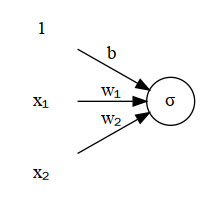
\includegraphics[width=0.4\textwidth]{./plots/neuron.gv.png}
%\label{fig:neuron1}
\end{subfigure}
\begin{subfigure}[b]{0.45\textwidth}
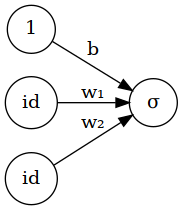
\includegraphics[width=0.4\textwidth]{./plots/neuron.2.gv.png}
\end{subfigure}
\caption{Two graphical descriptions of the neuron
$\sigma(w_1x_1 + w_2x_2 + b)$}. Here the bias $b$ is explicitly shown
but usually it is not depicted. In the left the variable names are explicitly
shown, while in the right they are not.
\label{fig:neuron2}
%\end{framed}
\end{figure}

Connecting many neurons together can create powerful parameterized
functions which we call neural networks.
%Connecting means that the output of one neuron is the input to one of the
%variables of a different neuron.
In feed forward networks the information only goes in one direction (no
feedback) and as we will see it means the network is a directed acyclic graph.

\begin{mydef}
\label{def:NN}
A \emph{feed forward neural network (NN)}is a \textbf{parameterized} map $\phi$
recursively defined
follows:
\begin{enumerate}
\item{} 
Activation functions ($1$, $id$, and $\sigma$) are NNs which are called the
\emph{elementary neurons} and they have no parameters ($\w=\emptyset$).
\item{} neurons are NNs
\item{} If $\psi :\R^n \to \R^m$ is a parameterized linear map then it is a NN.
\item{} If $\psi : R^n \to \R^m$
and $\rho: \R^m \to \R^l$ are NNs and their parameter sets are disjoint then $\phi = \rho
\circ \psi$ is a NN.
\item{} if $\nu:\R^n \to \R^m$ is a NN
and if $\psi_i: \R^{k_i} \to \R^{n_i}, i =1 \dots l$ are NNs, such that
$\sum_1^l n_i = n$
%and if $\psi_1, \dots \psi_n$ are NNs,
and if the parameter set of $\nu$ is disjoint from the combined parameters of
the $\psi_i$'s then
$\phi = \nu(\psi_1, \dots, \psi_n)$ is a NN
%if the dimensions "make sense".
.
\end{enumerate}

The parameter set $\w$ is called the \emph{weights} of $\phi$. Often we don't
distinguish between the network $\phi$ and its weights, and we identify both as
$\phi$.

In the definition we made the range and domain to be the entire $\R^n$ but it is
not necessary, we just need for the composition to be valid.
\end{mydef}

Feed forward neural network are depicted as a directed acyclic graph where every
node (with its incoming edges) corresponds to a neuron. You can think of
figure~\ref{fig:neuron2} left as depicting the neuron "component" in a network,
while figure~\ref{fig:neuron2} right shows a neural network description of
single neuron, comprised from elementary neurons.

If rule 5 of the definition~\ref{def:NN} is not used in the construction of
$\phi$, then the resulting network is hierarchical. Its graph can be partitioned
into \emph{levels} $l_0, l_1\dots$ and there are only directed edges between two
consecutive levels $l_i \to l_{i+1}$ (see figure~\ref{fig:nn1}).

The label inside the neuron describes its activation function. In the diagrams,
we let $\sigma$ represent the sigmoid function. We represent the identity
function either by the name of the variable ($x_1$, $y$ etc.) it acts on or
simple by $id$.   We let the label $1$ represent the constant function. We need
the constant function because with it we can represent any affine map as a
linear map with the first input always clamped to $1$. But connecting $1$ to
every (non-input level) neuron would clutter the graph so it is not shown in
most diagrams but still implicitly assumed. A directed edge between neurons
means that the output of the neuron at the tail is multiplied by the edge weight
and assigned to the input variable of the neuron it connects to. A Node's output
is therefore only dependent on the output of its direct ancestral nodes (plus
the bias which is usually not shown). Input-level neurons (sources) have no
incoming edges and they represent the beginning of the computation. Output
neurons (sinks) have no outgoing edges and their output is the final result of
the computation.

\begin{figure}[h]
%\begin{framed}
\centering
\begin{subfigure}[b]{0.5\textwidth}
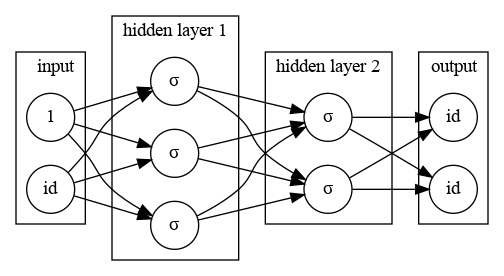
\includegraphics[width=0.8\textwidth]{./plots/neuronlayers.gv.png}
\end{subfigure}
\begin{subfigure}[b]{0.5\textwidth}
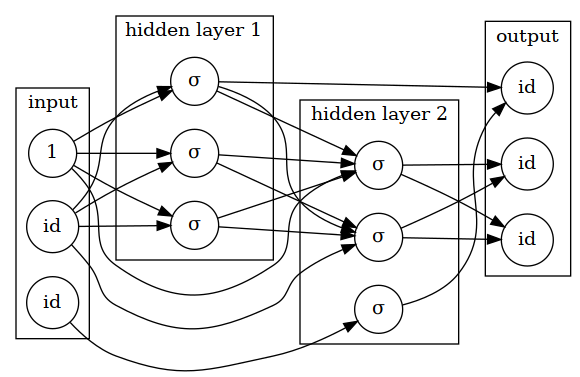
\includegraphics[width=0.8\textwidth]{./plots/neuronlayers.2.gv.png}
\end{subfigure}
\caption{The network in the top didn't use rule 5~\ref{def:NN} in the construction.
It is strictly hierarchical and there are only edges between nodes of two
consecutive layers. The one on the bottom is more general.
}
\label{fig:nn1}
%\end{framed}
\end{figure}

It turns out~\cite{nielsen2015neural} that the feed forward neural networks with
a single type of non-linear activation (e.g. sigmoid) and a single hidden layer
are "universal"; Which means that any continuous function $f$ can be uniformly
approximated by a feed forward neural network with a single hidden layer and
Sigmoid as the non-linear activation function. More precisely, let $B \subseteq
\R^n$ be a bounded domain. Let $f : B \to \R^m$ be continuous, and let $\epsilon
\in (0,1)$. Then there is a feed forward neural network with a single hidden
layer $\phi = \phi_{\w}$ and there is some value assignment for the parameters
$\w$ such that $(\forall \x \in B) \|\phi(\x) - f(\x)\|_2 \lt \epsilon $. The
size of that single hidden layer (the number of parameters) depends on $f$ and
$\epsilon$.

In the definitions we only used linear maps to grow the network. There are other
types of maps which are used, most commonly are convolutions but the principles
and the graphical description remain essentially the same.

There are additional types of parameterized functions which are used "within the
layer" such as batch normalization but we won't get into that as this is not a
thesis about neural networks per se.

\begin{figure}[h]
%\begin{framed}
\centering
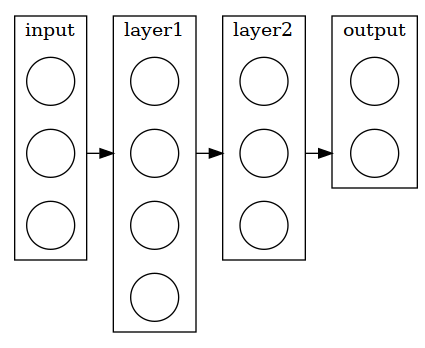
\includegraphics[width=0.5\textwidth]{./plots/multilayer.gv.png}
\caption{
A graph of a hierarchical feed forward neural network where the connections 
are abstracted. Edges between layers may represent in this case a fully
connected layer (every neuron has incoming edges from all neurons of the
previous layer) but it could also be used for describing a convolution.
}
\label{fig:nn2}
%\end{framed}
\end{figure}

As figure~\ref{fig:nn1} shows, 
The input layer is the where the input $(\x)$ is "fed in" and the output layer
is the final result of the evaluation $\phi(\x)$.
We call all the layers (or neurons) that are 
not in the input level or the output level "hidden"
because we don't usually know what is the input/output value in these.

\section{Loss functions}

In the claim about neural networks being "universal" in terms of approximating
function $f(\x)=\y$ with neural network $\phi(\x)$. We stated specifically
convergence in terms of $l_2$ norm $\|\phi(\x) - \y \|_2$, but the claim holds
in theory and in practice with other types of "distance-like" functions which we
call loss functions.

Moreover we usually don't know what is the function $f$ which we try to
approximate. Rather we are given paired samples of input/target $(\x, \y)$ and
we try to minimize the total error.

\begin{mydef}
\label{def:lossfunc}
Let $\phi :\R^n \to \R^m$ be a neural network.
A \textit{loss function} is a differentiable
function $\mathcal{L} : \R^{m}\oplus\R^m \to \R$. 
With "distance-like quality".
\end{mydef}

Typically the loss function is additive on the dimension, meaning it has the
form $(\forall \y,\z \in \R^m) \mathcal{L}(\y, \z)) = \sum_{i=1}^m \psi(y_i,
z_i))$

Let $\X \in \R^{N \times n}, \Y \in \R^{N \times m}$ be the input and the target
set and let $(\x,\y)$ be a paired input/target. We use the loss function
$\mathcal{L}$ as the target function for the minimization problem, $\min_{\w}
\sum_{(\x,\y)}\mathcal{L}(\phi(\x), \y)$ where the sum goes over all paires ($N$
rows)  (input, target).


For example $\mathcal{L}(\y, \z)) = \|\y - \z\|_2^2 = \sum_i |y_i - z_i|^2$ is a
one such loss function (the square error).

So far we defined $\phi$ and $\mathcal{L}$ on single input/target data points
$\x$ and $\y$. But we are interested in minimizing the total error
$\mathcal{L}(\phi(\X),\Y)$. So first we need to state how these functions
operate on sets of samples (matrices) rather than on data points (vectors).

Usually evaluation over the entire dataset is infeasible. Instead computation is
performed on batches, which are relatively small chunks of the data.

\begin{mydef}
\label{def:batch}
Let $\bv{X} \in  \R^{N \times n}$ be a data matrix. A \emph{batch}
$\bv{x} \in \R^{b \times n}$ is any subset of $b$ rows of $\bv{X}$
(Note that in this case $\x$ represents a matrix).
\end{mydef}

Batch $\x = \{\x_1, \dots \x_b\} \in \R^{b \times n}$ (row notation)
represents a subset of $b$ samples out of the total of $N$ samples in the
dataset.
Extending $\phi$ to operate on batches is trivial.
$\phi(\x) = \{\phi(\x_i)\}$ is the matrix where $\phi$ is applied on the rows of
the batch.
Given an input batch $\x$ and corresponding target batch of $\y$,
We extend the loss function to batches by averaging over the batch:
$\mathcal{L}(\phi(\x), \y) \triangleq \frac{1}{b} 
\sum_{i=1}^b \mathcal{L}(\phi(\x_i), \y_i)
$

\begin{mydef}
Let $\phi$ be a neural network as defined in~\ref{def:NN} and let $\mathcal{L}$
its associated loss function as defined in~\ref{def:lossfunc}---over vectors.
Let $\x = \{\x_1, \dots , \x_b\} \in \R^{b \times n}$ be a $b$-batch (in row
notation)
, and let $\y = \{\y_1, \dots , \y_b\} \in \R^{b \times m}$ be a corresponding
target batch.
Then $\phi$ and $\mathcal{L}$ \emph{extended} over batches are:
\begin{IEEEeqnarray}{C}
\phi(\bv{x}) \triangleq \{\phi(\bv{x}_i)\}_{i=1}^b \in \R^{b \times m}\\
\label{eq:NNbatch}
\mathcal{L}(\phi(\x), \y) \triangleq \frac{1}{b}\sum_{i=1}^b \mathcal{L}(\phi(\x_i), \y_i) \in \R
\label{eq:NNbatchloss}
\end{IEEEeqnarray}
\end{mydef}

If $\mathcal{L}$ is the square error function $\| \cdot \|_2^2$ on vectors, then
its extension to batches is $\frac{1}{b}\| \cdot \|_F^2$. The reason why we sum
and don't average over the dimensions will be cleared later when we get into
variational inference.

There is also a probabilistic way to interpret the total loss. We assume that
the data points $\X, \Y$ were randomly and independently sampled from the
unknown data distribution $p(\x, \y)$. Then equation~\ref{eq:NNbatchloss} can be
reformulated as the expected loss~\cite{bishop2006pattern}:

\begin{equation}
\mathcal{L}(\phi(\X), \Y) \approx
\mathrm{E}_{\x,\y \sim P(\x,\y)} \mathcal{L}(\phi(\x), \y)
\label{eq:NNbatchlossE}
\end{equation}

\section{Training}
This is just a brief explanation of the basic principals. Training deep networks
is a big subject which has many challenges and obstacles and a lot of
heuristics are used. 

Training the neural network $\phi_w$ means finding the weights that minimize the
loss function applied on the training input/target paired sets $\X,\Y$, in other
words minimizing $\min_{w} (\mathcal{L}(\phi_w(\X),\Y)$.
Usually we can't compute efficiently $\phi$ and $\mathcal{L}$ over the entire
sets because $N$ is too large, therefore we use batches.

\begin{mydef}
Let $\phi_{\omega}$ be a neural network and $\mathcal{L}$ its associated loss
function. And let $(\X, \Y)$ be our \emph{training set} consisting of 
the data matrix $\X$ and $\Y$
the corresponding target matrix.
Then \emph{Training} of $\phi_{\omega}$ with respect to $\mathcal{L}, \X$ 
means
algorithmically approximating the minimization problem:
\begin{equation}
\label{def:training}
\min_{\omega} \mathcal{L}(\phi_{\omega}(\X), \Y)
\end{equation}
\end{mydef}

During a \emph{training step} the network is applied on a batch $(\x,\y)$. Then the
loss function is applied on the output of the network and a gradient (with relation to the
weights) is taken using the efficient backpropagation
algorithm~\cite{nielsen2015neural}.
The gradient is used for the weight update rule, which
varies depending on the specific training algorithm. Typical training algorithms
are SGD (stochastic gradient decent) and Adam~\cite{jais2019adam},
which is the one used throughout
this work.

We only need to define the network, the loss function and the specific training
algorithm. The rest (derivation, weight update etc.) is taken care for us by the
backend of the software (Pytorch~\cite{pytorch2018pytorch}) and can be regarded
as a black box.

\subsection{Training, validation and testing data sets}

The data is partitioned into disjoint sets. The training set is used for the
training of the model. The testing set is used for the final performance
assessment. Sometimes a third subset, the validation set is used for tuning and
tweaking the model during training. The point is that the model "doesn't know"
the validation data because the weights are only trained on the training set,
but the hyper-parameters are optimized based on the validation set.
For example the validation set can be used for early
stopping during the training.
We didn't use a validation subset in our tests.
Finally the assessment is performed on the 
testing set which was completely held out during the training and
hyper-parameter tuning.


\subsection{Un/Supervised learning}

In unsupervised learning one seeks to "learn" or infer the target set $\Y$ (for example
category information) from $\X$ without seeing $\Y$ during training.
For example in the case of MNIST we want to teach the model to distinguish
10 categories of images corresponding to the $10$ digits, without having access
to the digit tags in the training set.

Supervised learning means the $\Y$ target information is fully accessible (every image
is tagged with the digit it represents). This is a much simpler classification
task.

Semisupervised learning is the hybrid case of both, where the training set
includes a small portion of known paired input/targets $(\x,\y)$ while for the
rest of the training set we only have $\x$ input and need to infer $\y$.
Semisupervised learning tasks often arise in natural situations. For example
there may be a large image data set where only a portion of the images have been
manually tagged.

\section{Autoencoders}

The basic type of an autoencoder which we informally call "vanilla" autoencoder
is a neural network that tries to "learn" the identity function. Though it sounds
pointless on a first thought, the point is how we construct this network. An
autoencoder consists of two neural networks.
An encoder network maps the input into a lower dimensional so called "latent
space", and a decoder network maps the latent space back into the high
dimensional input layer.
In the case of the vanilla autoencoder the target for the loss function is the
same as the input $\Y = \X$.

\begin{figure}[h]
%\begin{framed}
\centering
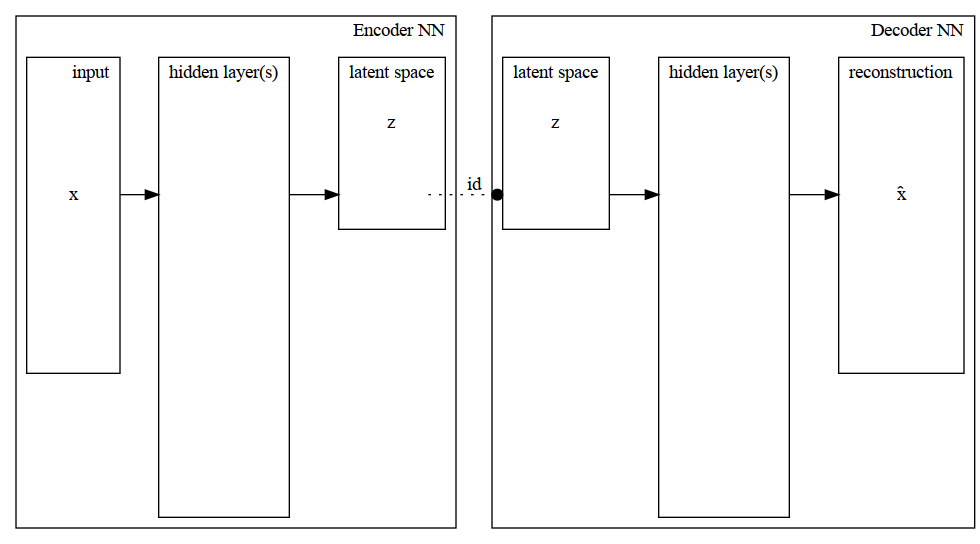
\includegraphics[width=0.8\textwidth]{./plots/autoencoderNN.gv.png}
\caption{
A graphic description of a "vanilla" autoencoder.
}
\label{fig:autoencoder}
%\end{framed}
\end{figure}

\begin{mydef}
\label{def:autoencoder}
An \textit{Autoencoder} (AE) is a pair 
$(\phi, \psi)$ of feed forward neural networks 
$\psi : \R^n \to \R^m, \nu : \R^m \to \R^n$.

$\psi$ is called the \emph{encoder} network, and $\nu$ is called the
\emph{decoder} network and the composition
$\phi = \nu \circ \psi$ is called the \emph{autoencoding network}. 

We call $\R^m$ or more genrally the domain of the decoder, \emph{the latent
space}, and $\R^n$ (or more generally the domain of the encoder) is called
\emph{the observed space}.

Given a batch $\x \in \R^{b \times n}$ we call $\z = \psi(\x) \in \R^{b \times m}$
the \emph{latent representation} of $\x$ or the \emph{encoding} of $\x$.
\end{mydef}

While the definition as is given is symmetric, it is assumed that $n > m$, and
therefore $\psi$ represents dimensional reduction (in other words encoding) of
the data and $\nu$ represents expansion back to original space (decoding).

The idea here is that the original high dimensional data can be embedded
in a low dimensional space by the encoder. The decoder then can reconstruct the
original data from the embedding.

There are many variations of autoencoders. For example a "denoising" autoencoder is
essentially that same model but it receives a "noisy" version of the input and
tries to reconstruct the original clean version.
We informally call the type of autoencoder of
definition~\ref{def:autoencoder} which aims to learn the identity function 
on the original input, and which is using the square error loss function, 
a "vanilla" autoencoder. 

\subsection{A word choosing latent space dimension and plotting it}
The dimension of the latent space is a hyperparameter of the model. It's choice
can affect the model's performance and its numerical stability.
We don't claim that we some sort of a system of how to choose it. For us it's a
matter of trial and error with some common sense. For example it should be in
the same order as PCA dimensions (which defaults on $50$). We usually choose
something in the range 8---64.

When it comes to plotting the latent space, one option is to set the dimension
on 2 or 3 so it can be plotted directly. This works ok for some datasets but
generally we need more freedom in choosing this value.
And in the higher dimension case, first we perform PCA on the latent space. Then
either directly plot the 2 or 3 most significant PCs, or use
UMAP~\cite{mcinnes2018umap}. UMAP seems to be the golden standard nowadays,
and it is used both in the machine learning as well as in the RNASeq
milieus.
For us UMAP is a black box that projects input into 2 dimensions relatively
faithfully and does it fast (unlike TSNE). 
In some other cases, we show UMAP of the input space $\X$ rather than of latent
space. In each image it should be stated which space and which projection is
used.

\subsection{Relation between PCA and AE}
For \textbf{centered} data, where every variable (column of $\bv{X}$)
has a sample mean of $0$, the first $k \leq \text{rank}(\bv{X})$ principle components
$\bv{P}$ are the solution for equation~\ref{eqn:pca}; Whereas a \textbf{linear}
autoencoder solves equation~\ref{eqn:pca3}. As mentioned, it must hold that $E =
D^{\dagger}$ (the encoder must be the Moore-Penrose inverse of the decoder).

A linear autoencoder with the  square error
loss function is almost equivalent to
PCA~\cite{plaut2018principal}; At the optimum, a bottleneck space of dimension $k$
is spanned by the first $k$ principle components of the input $\bv{X}$.
In general, an AE can be seen a PCA-like, but non-linear method for
dimensionality reduction.

\begin{figure}[h]
%\begin{framed}
\centering
\begin{subfigure}[t]{0.45\textwidth}
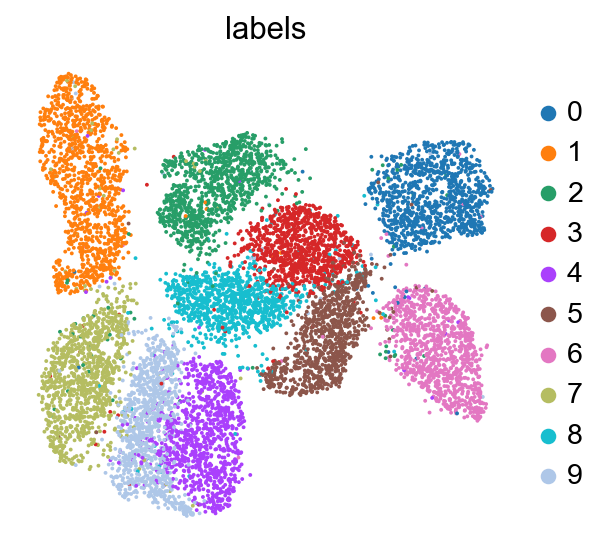
\includegraphics[width=0.95\textwidth]{images/pca.umap.mnist.png}
\caption{MNIST: UMAP of the PCA}
\end{subfigure}
\begin{subfigure}[t]{0.45\textwidth}
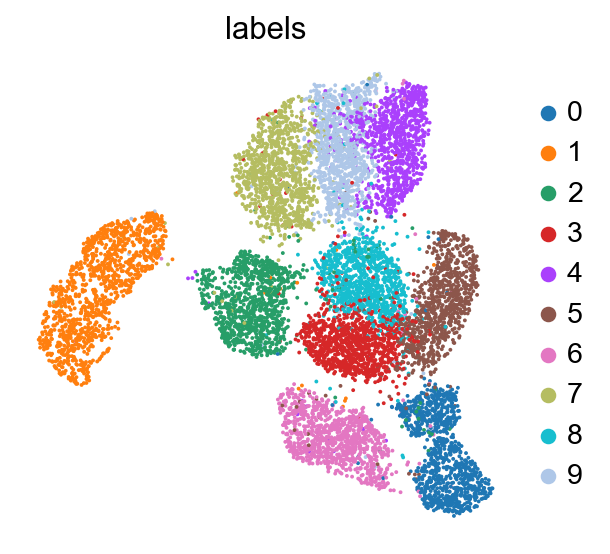
\includegraphics[width=0.95\textwidth]{images/ae.umap.mnist.png}
\caption{MNIST: UMAP of the AE}
\end{subfigure}
%\end{framed}
\caption{PCA (l) compared with "vanilla" autoencoder (r) on the MNIST dataset}
\label{fig:pcavae}
\end{figure}

Figure~\ref{fig:pcavae} shows on the left a
UMAP~\cite{mcinnes2018umap} of the principle components of the testing subset of
MNIST (images of hand written digits). On the left we see a UMAP of the latent
space encoded by the encoder of a "vanilla" autoencoder with the square error loss
function. The autoencoder was
trained on the training set and didn't "see" the testing images during training.
The results appear quite similar.


\nocite{martinunsupervised}
\nocite{kingma2013auto}
\nocite{szczurek2010introducing}

\printbibliography
\end{document}
